\documentclass[12pt,a4paper]{article}
\usepackage[utf8]{inputenc}
\usepackage[french]{babel}
\usepackage[T1]{fontenc}
\usepackage{amsmath}
\usepackage{amsfonts}
\usepackage{amssymb}
\usepackage{graphicx}
\usepackage{fourier}
\usepackage{caption} 
\usepackage{subcaption}
\usepackage{float}% importtant pour mettre les images sans espaces autour.
\captionsetup{font=small}
\usepackage[left=2cm,right=2cm,top=2cm,bottom=2cm]{geometry}
\title{Compte rendu de TP : Mod\'elisation de l'appareil photo des smartphones par une lentille mince.}
\author{BATHILY Ousmane \\ Universite Paris-Saclay}
\date{}
\begin{document}

\maketitle
L'objectif ici est de savoir si l'appareil photo d'un smartphone peut \^etre mod\'elis\'e par une lentille mince. Ce travail reposera ce que nous avons fait pendant 3 s\'eances : durant la premi\`ere nous effectuerons un travail th\'eorique en faisant le lien entre l'image, l'objet et les différentes caract\'eristiques de l'appareil photo. Nous conclurons cette première partie par une pr\'ediction qui devra \^etre test\'ee exp\'erimentalement lors de la deuxi\`eme s\'eance. La derni\`ere sera consacr\'ee au traitement des donn\'ees recolt\'ees lors de la s\'eance 2.
\section{S\'eance 1 : La cascade de Yellowstone}
\subsection{Introduction}
La probl\'ematique de cette premi\`ere partie est de d\'eterminer la hauteur de la cascade du Yellowstone en s'appuyant sur les deux photographies ci-dessous :
\begin{figure}[H]
\begin{center}
\includegraphics[scale=0.5]{Figures/yellow1.jpg}   
\caption{Photographie de la cascade de Yellowstone.}
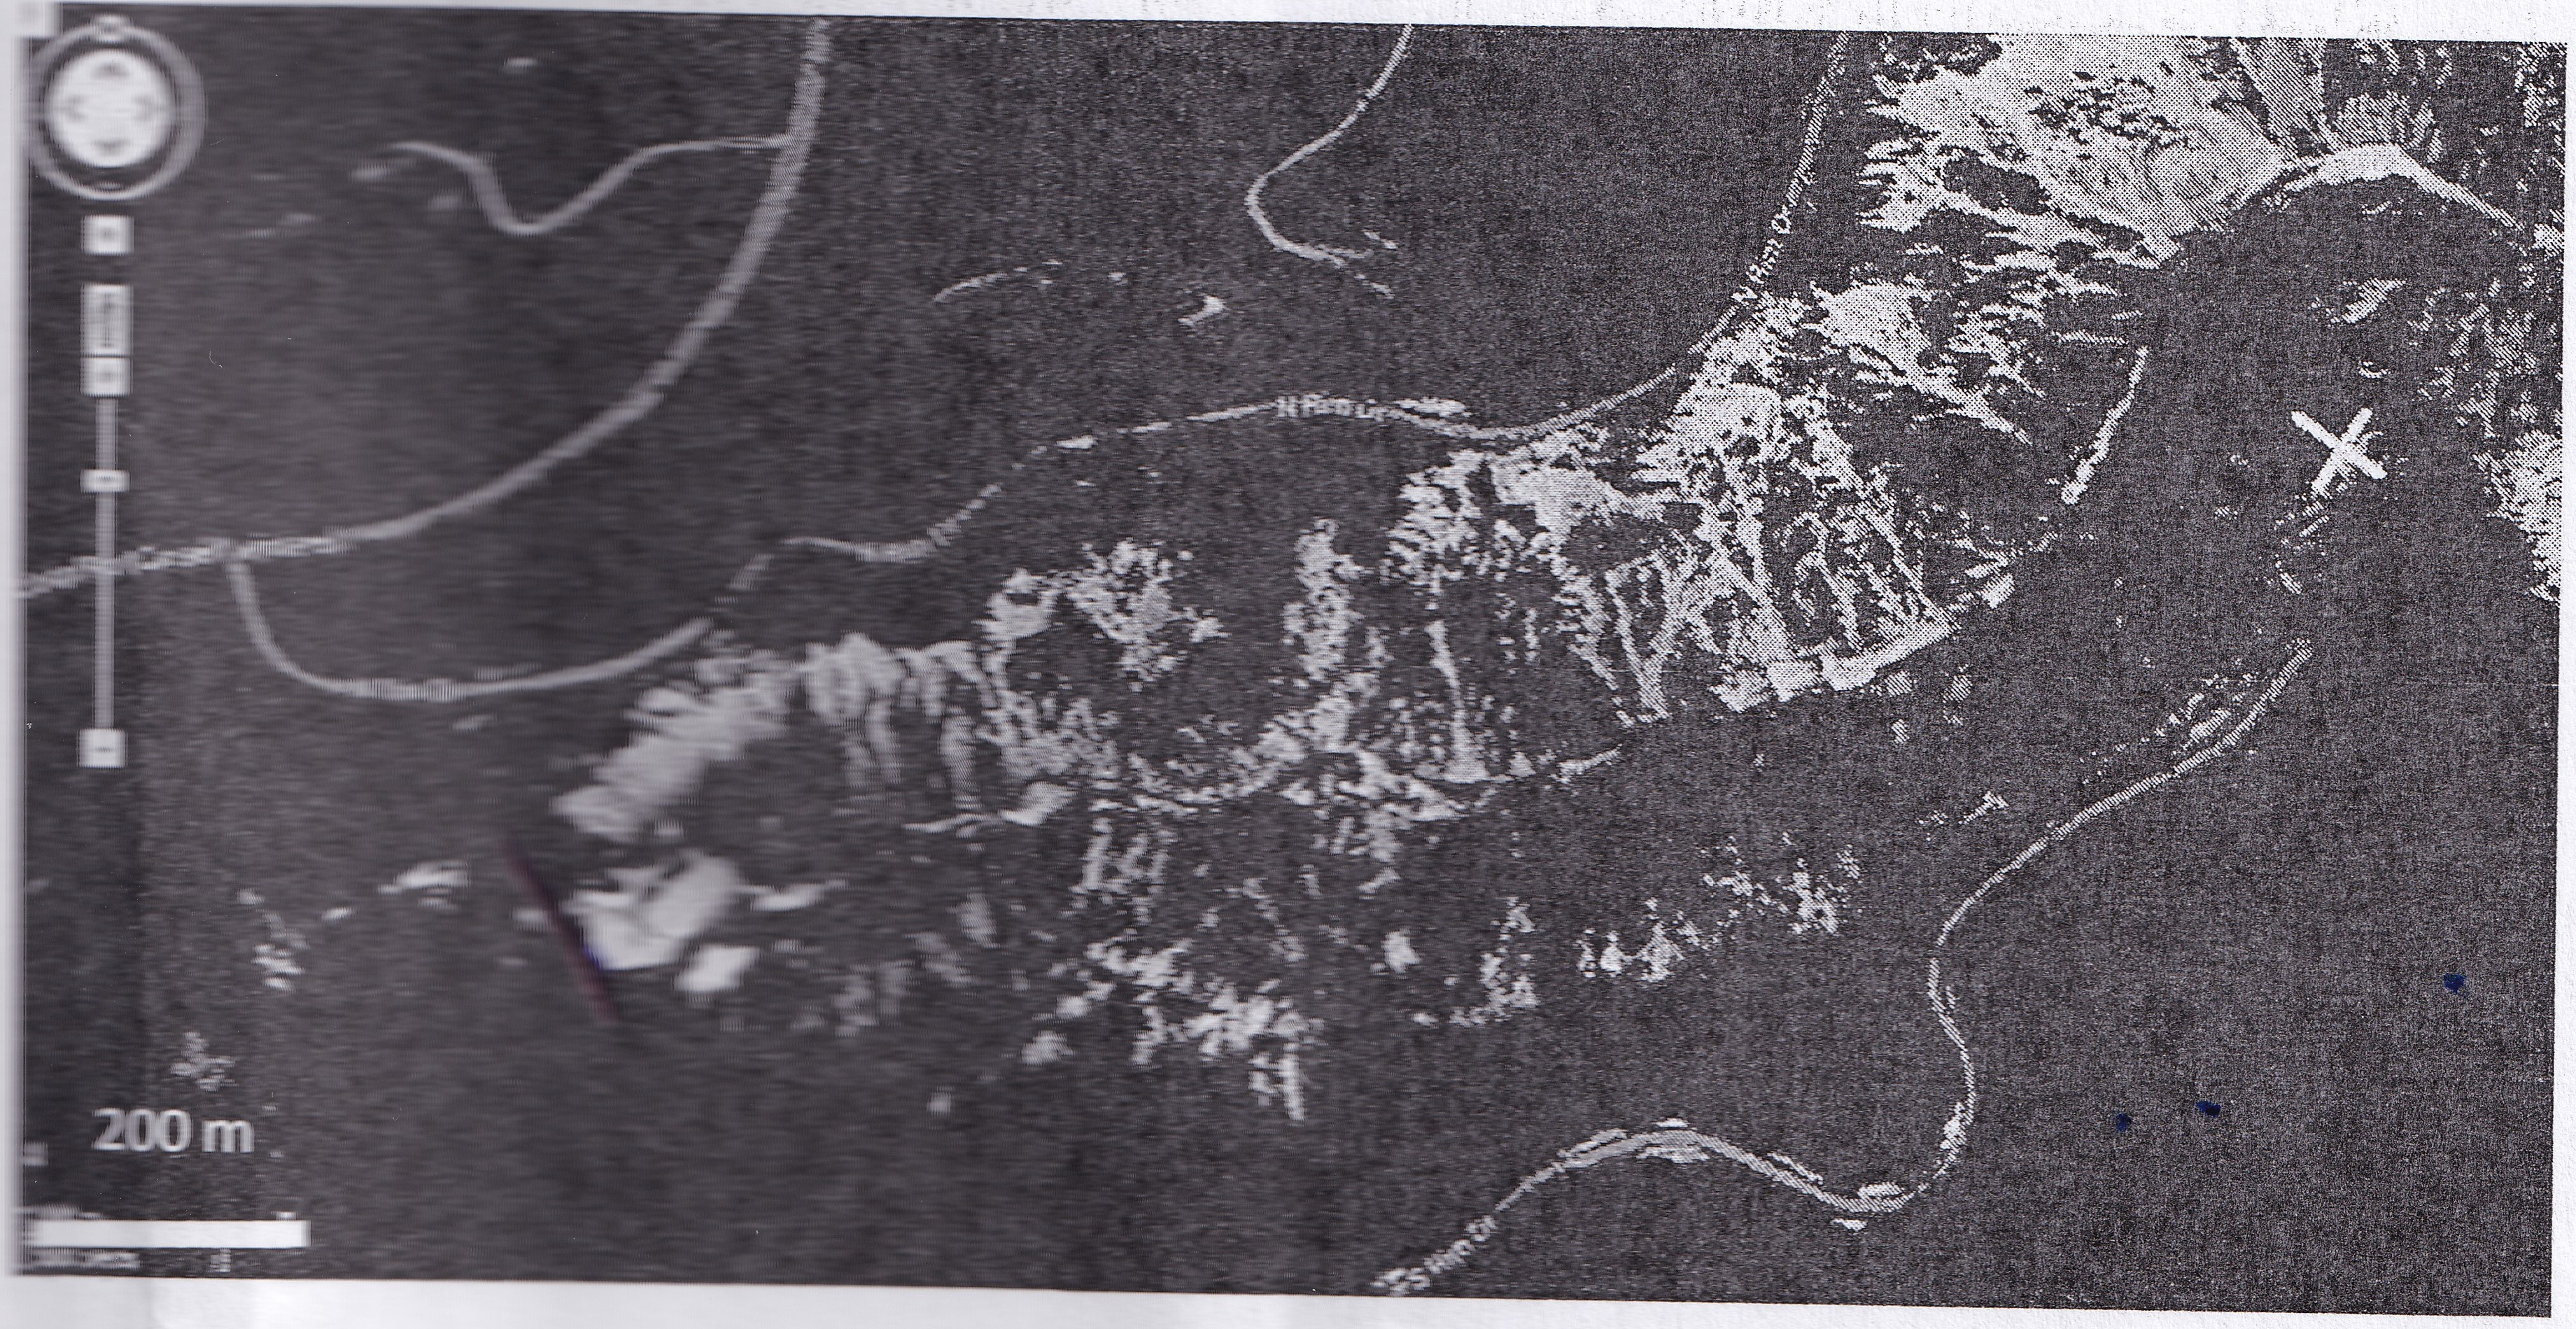
\includegraphics[scale=0.6]{Figures/yellow2.jpg}
\caption{Vue d'ensemble incluant la position du photographe(croix blanche) et la cascade de Yellowstone.}
\label{fig1}
\end{center}
\end{figure}

Pour répondre à cette question, nous allons tout au long de ces 4 séances utiliser les lois de l'optique géometrique en se focalisant sur le comportement de lentilles convergentes. On utilisera en particulier ces deux propositions : 
\begin{equation}
\frac{1}{\overline{OA'}} - \frac{1}{\overline{OA}} = \frac{1}{\overline{OF}},
\end{equation}
$\overline{OA}$ et $\overline{OA'}$ étant les mesures algébriques d'un objet et de son image et $\overline{OF}$ la distance focale.
\begin{equation}
\gamma = \frac{\overline{OA'}}{\overline{OA}}, \quad \text{$\gamma$~~l'agrandissement de l'image par rapport à l'objet.}
\end{equation}
\subsection{Démarche et grandeurs}
Grâce aux deux images précédentes nous allons pouvoir donner une estimation de la hauteur de la cascade en faisant le lien entre la hauteur réelle de la cascade, son image par l'appareil photo et sa hauteur sur la figure (1).
En considérant que la lentille de l'appareil peut être assimilée à une lentille convergente, voici un schéma de ce qu'il se passe au niveau de l'appareil photo :
\begin{figure}[!ht]
\begin{center}
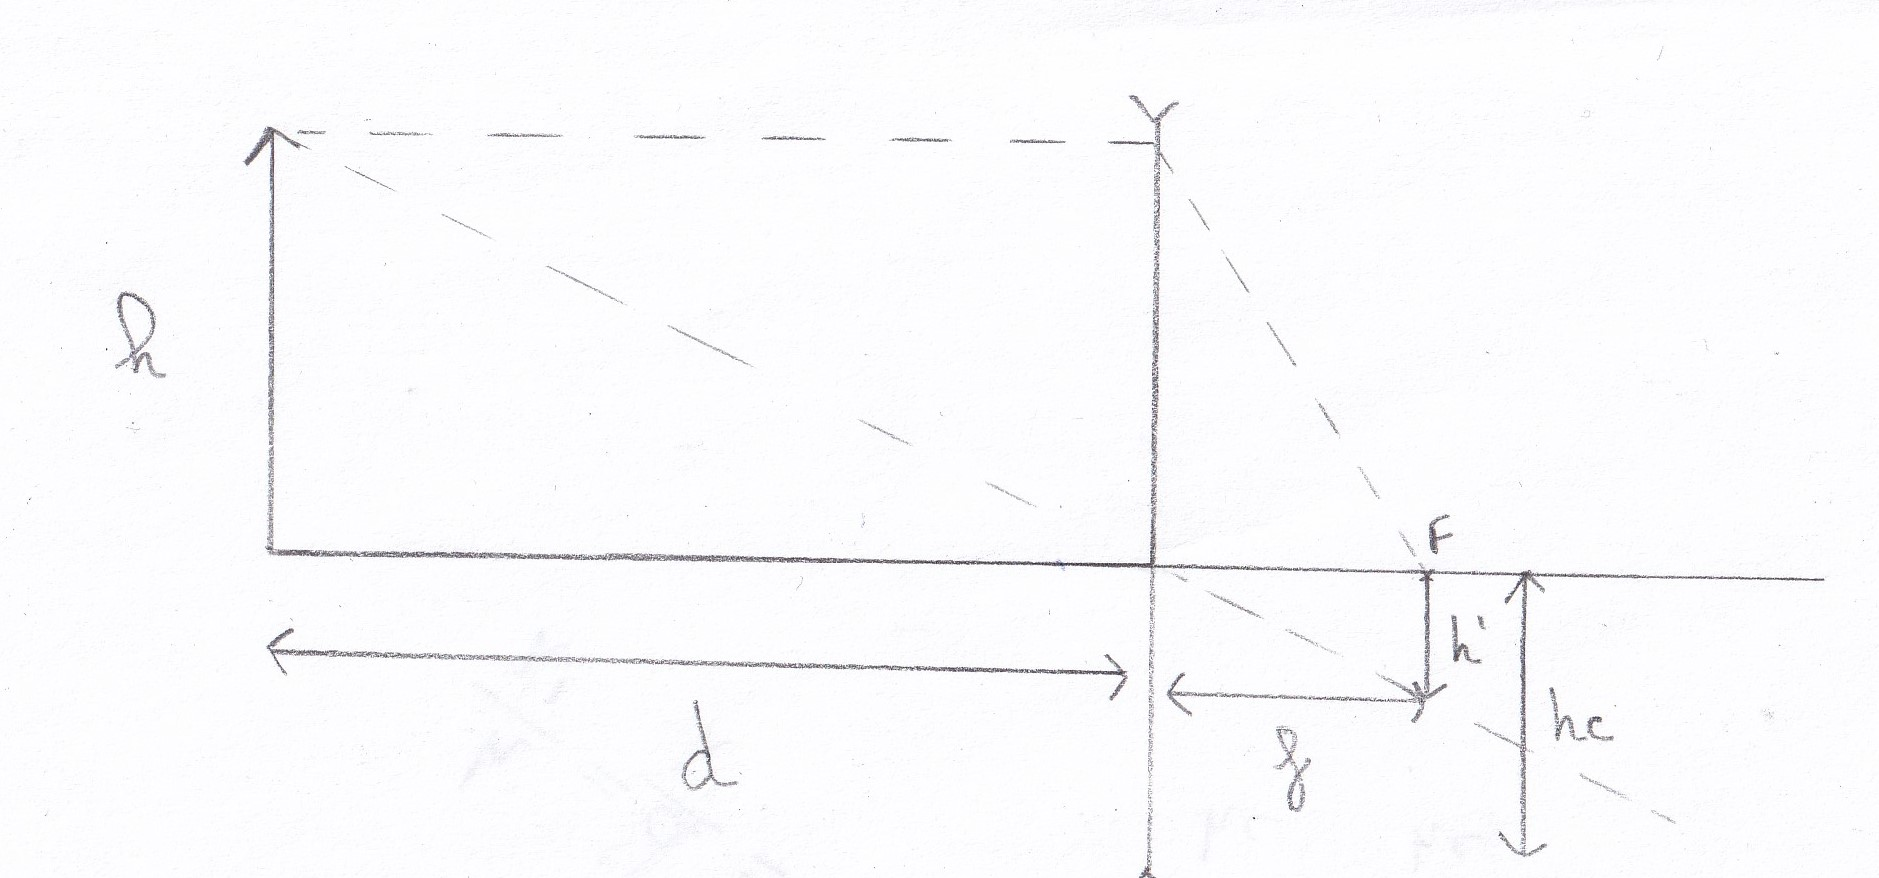
\includegraphics[scale=0.6]{Figures/schéma1.jpg}   
\caption{Modèle de l'appareil photo}
\end{center}
\end{figure}

Voici maintenant la liste des grandeurs que nous allons utiliser tout au long de la résolution de ce problème :\\
\begin{itemize}
\item $h :$ la hauteur réelle de la cascade que nous cherchons à approximer;
\item $d :$ la distance séparant le photographe de la cascade, que nous pouvons mesurer à l'aide de la figure (2) en s'appuyant sur l'échelle qui nous est donnée;
\item $f :$ la distance focale de l'appareil qui nous est donnée valant 135 $mm$;
\item $h' :$ l'image de la cascade par la lentille convergente de centre O qui peut être déterminer à l'aide la relation de conjugaison (1);
\item $hc :$ la hauteur du capteur de l'appareil photo qui nous est aussi donnée valant 14.9 $mm$;
\item $h''$ : la hauteur de la cascade sur la photo, valant $7~cm$;
\item $he$ : la hauteur totale de la photographie , valant $10.8~cm$;
\end{itemize}

On a : 1,7 cm (photo) $\longrightarrow$ 200 m et la distance $d$ représentée sur la photo vaut 11 cm.
Avec un simple produit en croix, on en déduit que $d = (11\cdot10^{-2})/1.7\cdot10^{-2} = 1.3\cdot10^3$ $m$. L'incertitude sur les mesures de distance à la règle graduée est $\Delta d = 5\cdot10^{-4}~m$

\begin{figure}[H]
\begin{center}
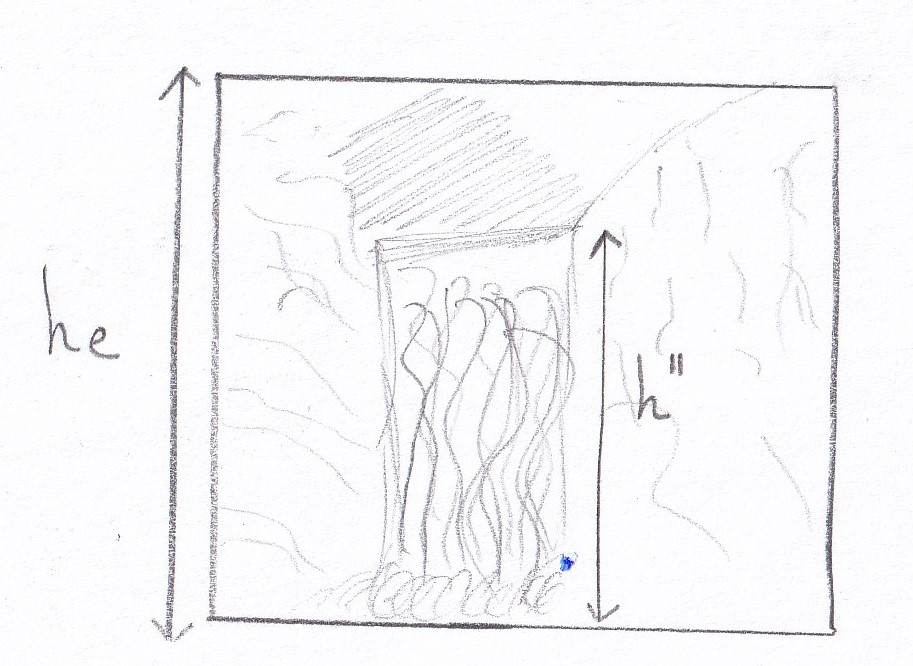
\includegraphics[scale=0.8]{Figures/schéma2.jpg}   
\caption{L'agrandissement $\gamma$ reliant aussi la hauteur de l'écran $he$ et la hauteur de la cascade sur la photo $h''$}
\end{center}
\end{figure}

\subsection{Résolution de problème}
Grâce à la connaissance de $h''$ et de $he$, nous pouvons en déduire l'agrandissement qui est responsable des dilatations des grandeurs $h''$ et $h'$, on a donc : 

\begin{equation}
\gamma=\frac{hc}{h'} = \frac{he}{h''} \Longleftrightarrow h' = \frac{h''hc}{he}
\end{equation}
D'après la figure 3, les constructions nous suggèrent que par le théorème de Thalès, nous avons : 
\begin{equation}
\frac{h}{h'}=\frac{d}{\overline{OA'}} \Longleftrightarrow h = \frac{dh'}{\overline{OA'}}
\end{equation}
, avec $\overline{OA'}$ la distance algébrique séparant le centre optique de l'image $h'$. D'après (1), on a :\\ $$\frac{1}{\overline{OA'}}-\frac{1}{d} = \frac{1}{f} \Longleftrightarrow \overline{OA'} = f, \quad (d\ggg OA')$$
On en déduit d'après (3) et (4) : 
\begin{equation}
\boxed{h = \frac{dh''hc}{hef}}
\end{equation}
\\
Vérifions l'homogénéité de l'expression que venons de déterminer : $[h] = \frac{[L^3]}{[L^2]} = [L]$, h est donc bien homogène à une longueur.\\
\\Calculons maintenant l'incertitude sur $h$ avant de passer à l'application numérique. Les valeurs de $f$ et de $hc$ nous ont été données sans leurs incertitudes, la valeur de $\Delta h$ sera sous-estimée.\\ \\ En utilisant la méthode de la dérivée, qui semble la plus adapté dans notre situation (erreurs non indépendantes), on a : $$ \Delta h = \Delta d\left(\left\lvert \frac{\partial n}{\partial d} \right\rvert + \left\lvert \frac{\partial h}{\partial h''} \right\rvert + \left\lvert \frac{\partial h}{\partial he} \right\rvert\right)= \Delta d\left(\frac{h''hc}{hef}+\frac{dhc}{hef} + \frac{dh''hc}{he^2f}\right) = \frac{\Delta dhc}{hef}\left( h''+d + \frac{dh''}{he}\right) $$ 
Passons maintenant à l'application numérique : \\
$$\Delta h = \frac{5\cdot 10^{-4}\cdot 14,9\cdot 10^{-3}}{10,8\cdot 10^{-2}\cdot 135\cdot 10^{-3}}\cdot \left( 7\cdot 10^{-2} + 1,3\cdot 10^{3}+\frac{7\cdot 10^{-2}\cdot 1.3\cdot 10^{3}}{10,8\cdot 10^{-2}}\right) = 1.09~m $$
On a finalement : $$h = \frac{1,3\cdot 10^{3}\cdot 7\cdot 10^{-2}\cdot 14,9\cdot 10^{-3}}{10,8\cdot 10^{-2}\cdot 135\cdot 10^{-3}} = 92,9  m$$, soit :$$\boxed{h = (92,9 \pm 1.09)~m }$$
\subsection{Conclusion et discussion}
Concernant le hauteur que nous venons d'estimer, elle semble cohérente quand on sait que la cascade mesure en réalité à peu près 100 mètres, l'incertitude semble raisonnable aussi. Nous ne savons rien quant à l'inclinaison du capteur par rapport à la cascade, qui est un élément important lors de l'estimation de la hauteur d'une cascade.\\

Cette première séance nous a permis faire le lien entre les grandeurs caractéristiques lors de l'étude des lentilles minces.
Par conséquent si l'appareil photo d'un smartphone obéi à la loi donnée par l'équation (5), alors nous pouvons considérer qu'il est assimilable à une lentille mince et c'est justement ce que nous allons essayer de mettre en évidence lors des deux autres séances.
\section{Séance 2 : Mesurer la focale de l'appareil photo de notre smartphone}
\subsection{Introduction}
Nous allons ici proposer une expérience permettant de vérifier le modèle établi durant la partie précédente. Nous disposons d'un smartphone doté d'un appareil photo numérique, de focale $f = 4mm,$ (28$mm$ effective), d'une ouverture  $hc=0.3$ pouces $= 8.5 mm$ et dont la taille de l'écran vaut : $he~=~5.5~in = 13.97~cm$. Les informations données sont issues du site \underline{gsmarena.com}.
\begin{figure}[H]
\begin{center}
\includegraphics[scale=0.3]{Figures/écran.png}
\\
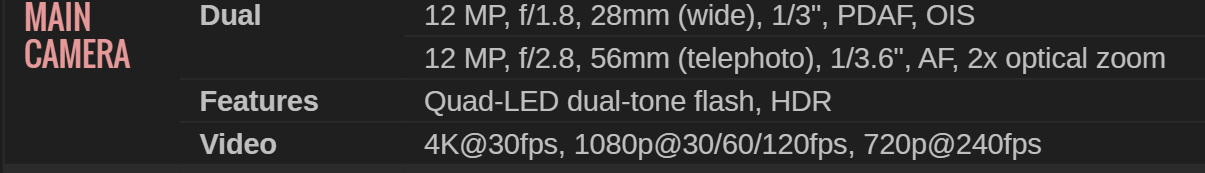
\includegraphics[scale=0.3]{Figures/photo.png}
\caption{Information sur l'appareil photo et l'écran du smartphone}
\end{center}
\end{figure}
Nous avons donc accès aux grandeurs "fixes" de l'appareil photo et une idée serait de faire varier la distance $d$ séparant l'appareil photo d'un objet de taille constante $H$ et de suivre l'évolution du rapport $H/h''$ . En effet, d'après l'équation (5) on a  : \\
\begin{equation}
H = \frac{dh''hc}{hef} \Longleftrightarrow \frac{H}{h''}~=~d\cdot \frac{hc}{hef} = d\cdot K \text{, en posant $K = \frac{hc}{hef}$}.
\end{equation}
\subsection{Protocole expérimental}
Il s'agira donc de faire varier $d$ et de mesurer la hauteur de l'image sur l'écran $h''$ en sachant $H$ et $K$ constants, puis de tracer l'ensemble des points tel que $\frac{H}{h''} = f(d)$. Si l'appareil photo est assimilable à une lentille mince alors la relation sera linéaire avec comme coefficient directeur le nombre K. Nous allons donc réaliser une série de mesures et voici la liste du matériel dont nous aurons besoin :
\begin{itemize}
\item un objet de hauteur $H$, ici une bouteille de hauteur $H~=~24.5~cm$;
\item un support permettant de garder le smartphone et l'objet parallèle;
\item du scotch, afin de maintenir bien droit le téléphone et le support entre deux mesures successives ;
\item une règle graduée;
\end{itemize}

\begin{figure}[H]
\begin{center}
\subcaptionbox{A notre échelle}
	{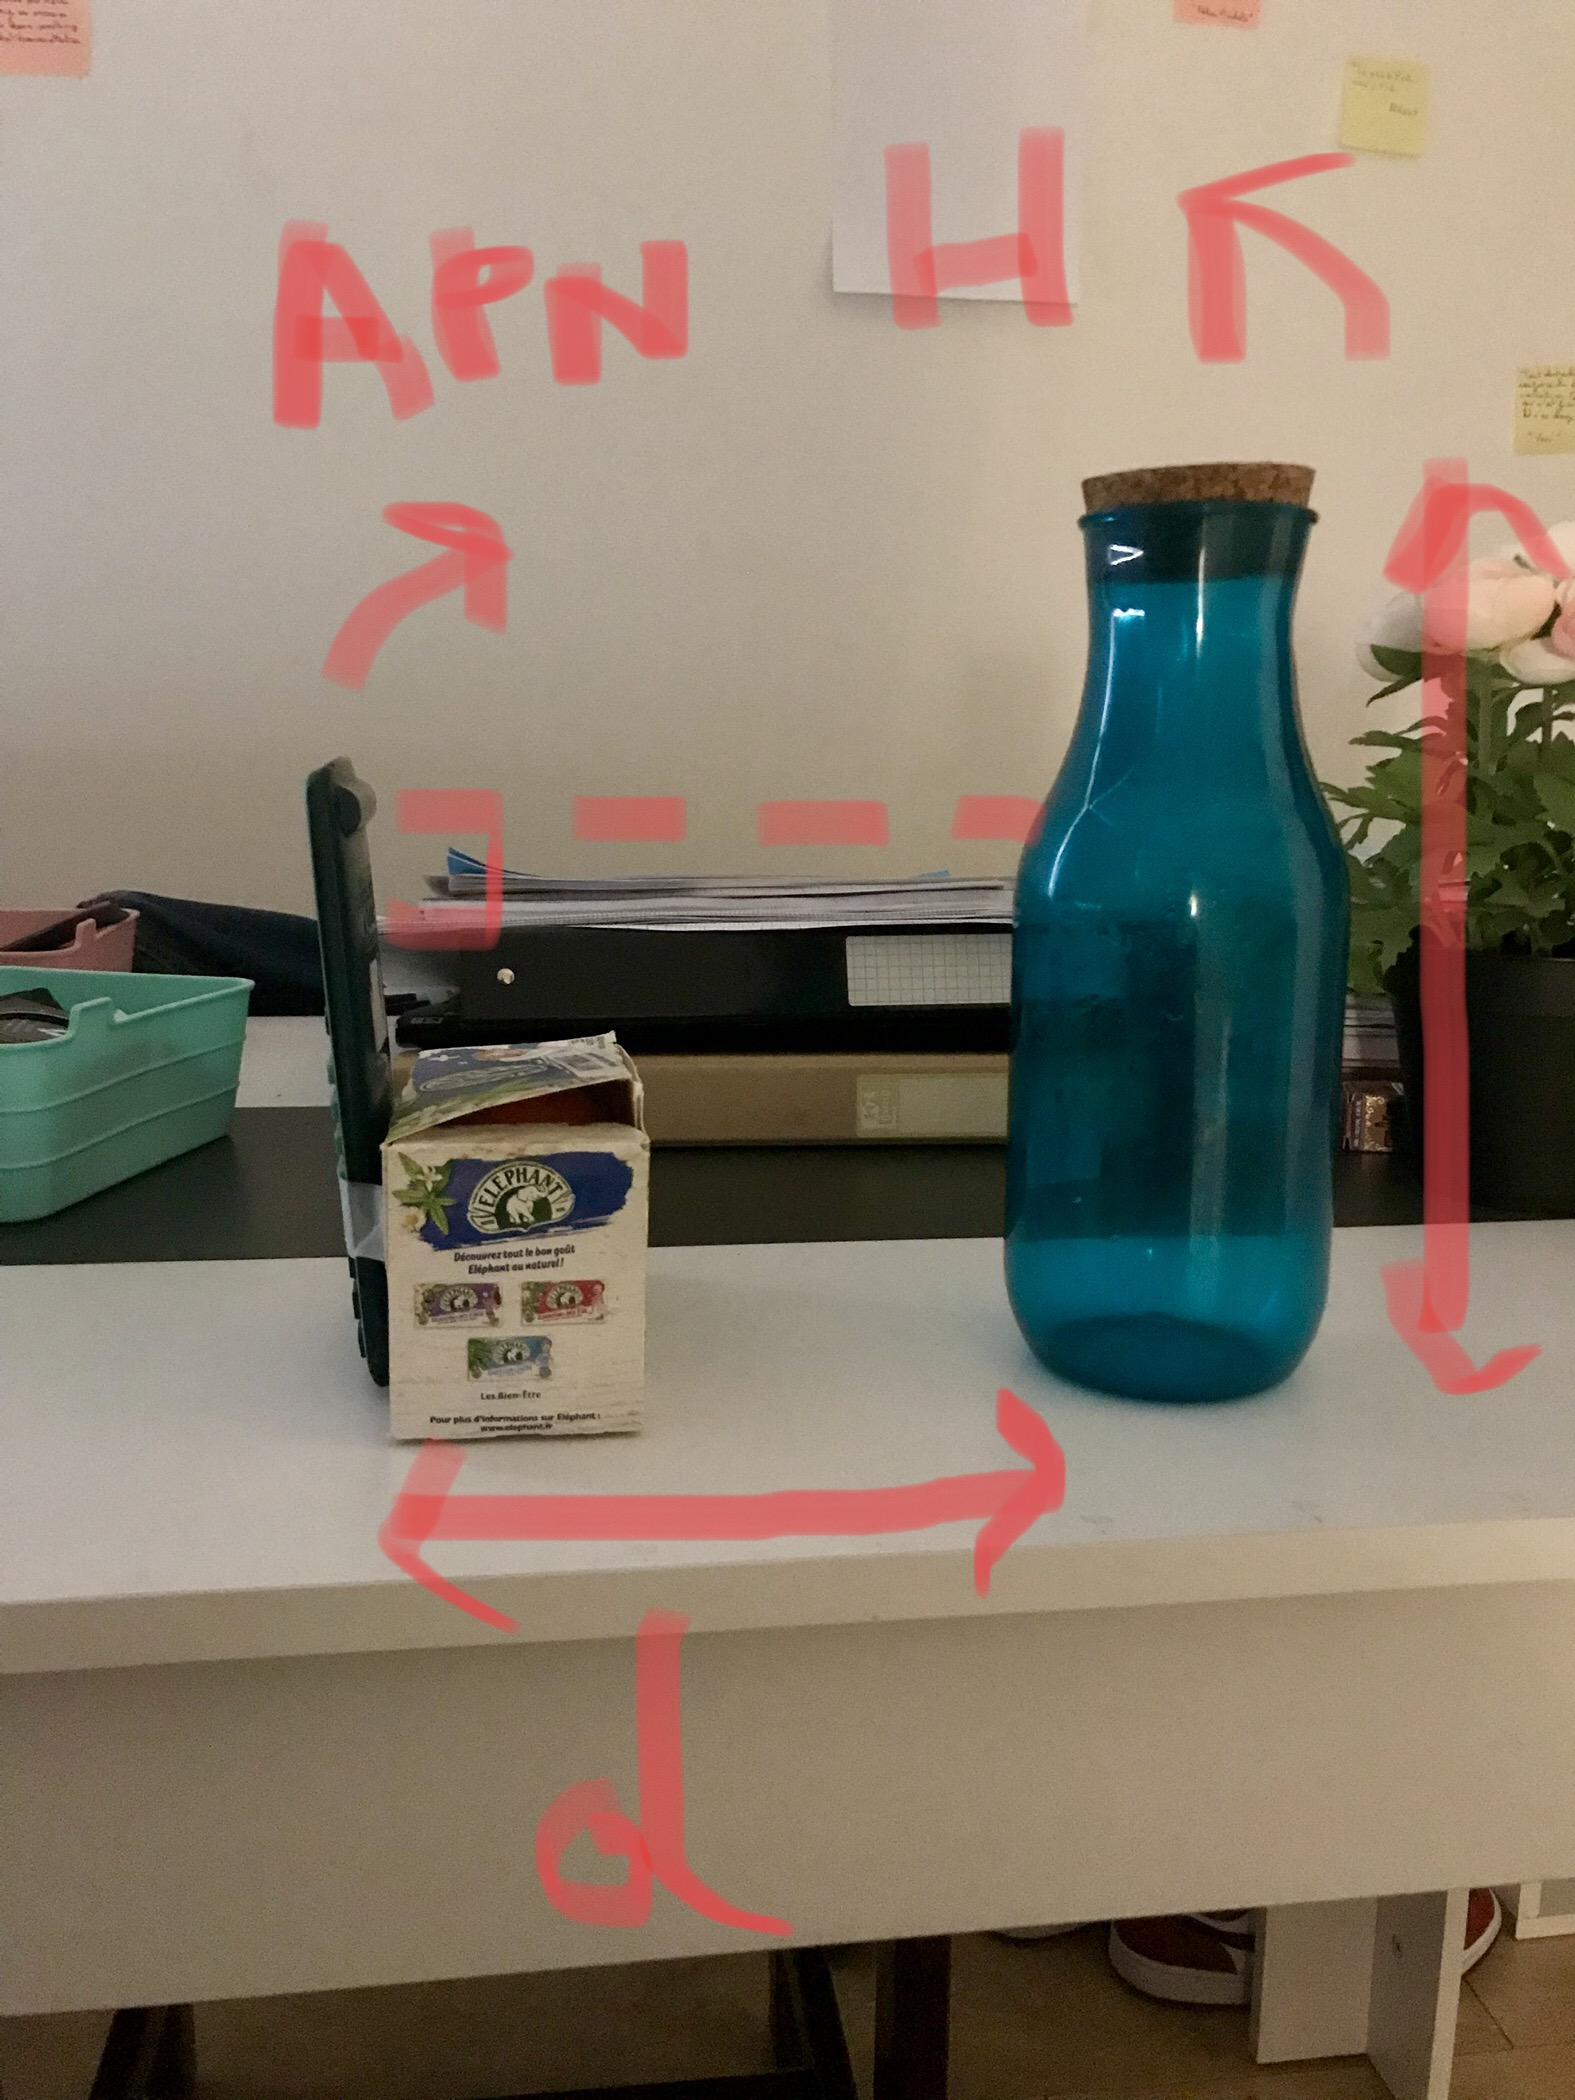
\includegraphics[scale=0.125]{Figures/s1.jpg}}
\hspace*{\fill}
\subcaptionbox{Au niveau de l'écran}
	{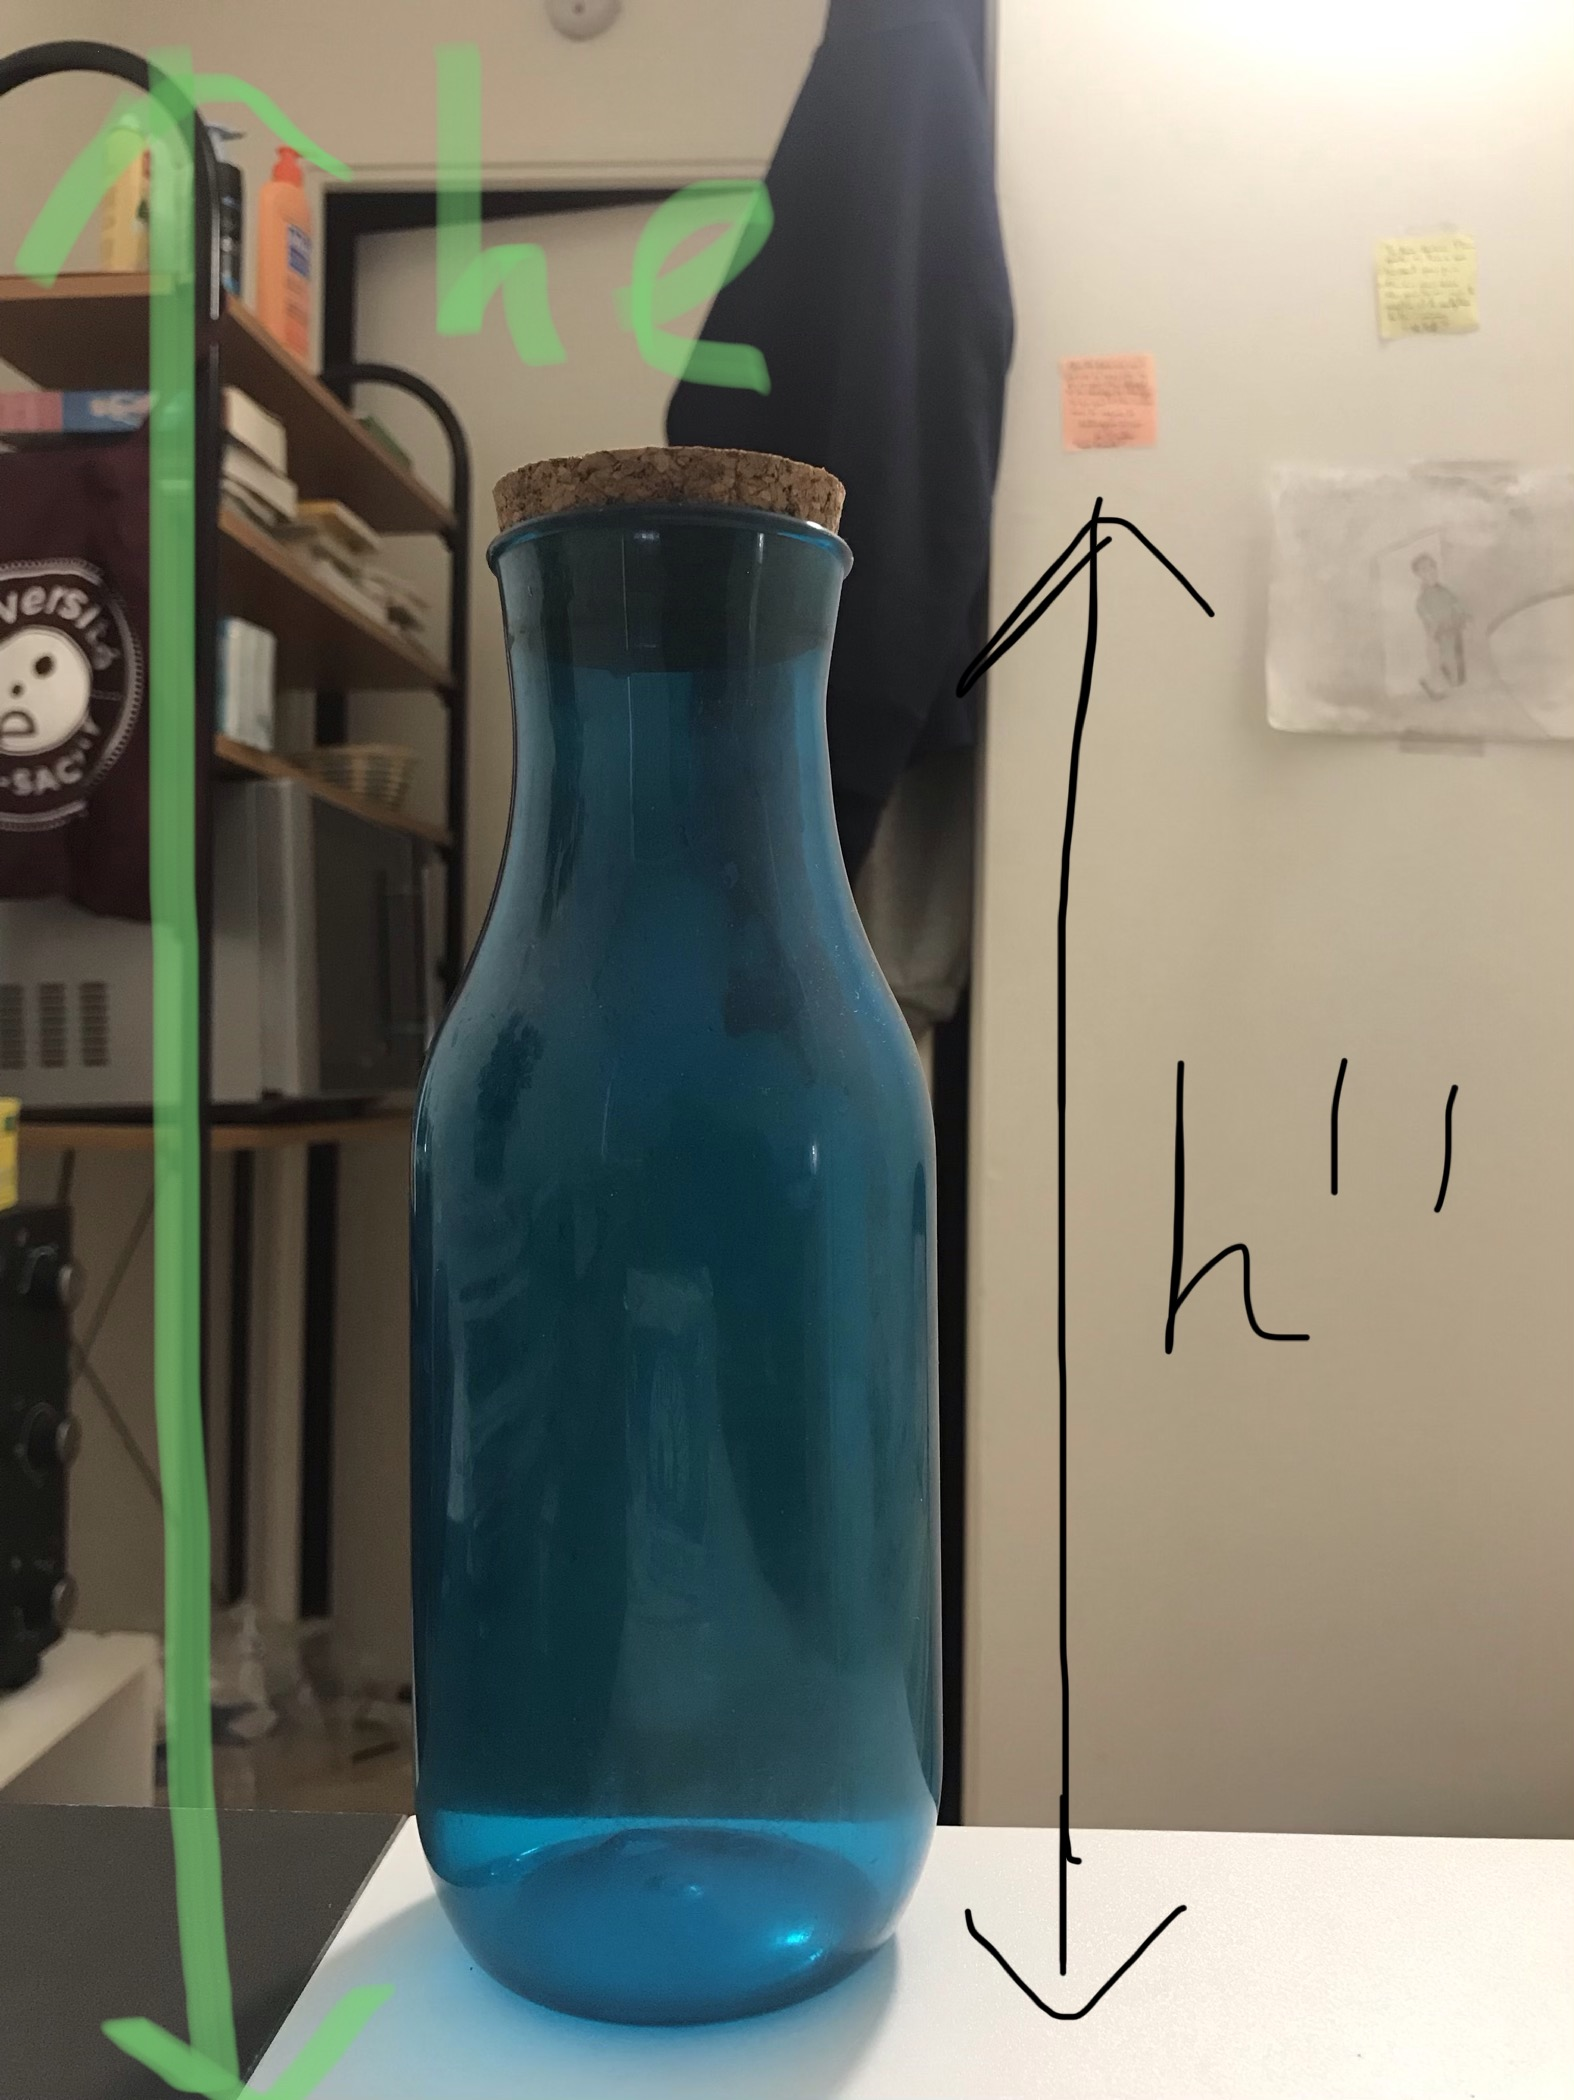
\includegraphics[scale=0.125]{Figures/s2.jpg}}
\caption{Schéma représentant les différentes grandeurs relatives à notre expérience}
\end{center}
\end{figure}
Dans la section \textbf{1.1}, nous avions dis que nous utiliserions les lois de l'optique géométrique et on rappelle que lors de l'élaboration d'un modèle physique quelconque, il est important de discuter des hypothèses et conditions sous lesquelles le modèle est valable. Pour l'optique géométrique nous devons vérifier que les objets interagissant avec la lumière ont des dimensions bien supérieurs à la longueur d'onde des rayons lumineux. On  peut essayer de comparer la taille de l'ouverture $hc$ qui est de l'ordre du millimètre aux longueurs d'ondes $\lambda$ associées à la lumière visible (quelques centaines de nanomètres). Qualitativement, on voit bien que $\lambda \ll hc$, nous ne serons donc pas embêter par les phénomènes de diffraction ou d'interférences, ouf ! \\
 

L'incertitude sur les mesures à la règle graduée reste la même soit $\Delta d = 5\cdot 10^{-4}m$. Calculons maintenant l'incertitude sur $H/h''$, en utilisant encore une fois la méthode de la dérivée :$$
\Delta(H/h'')= \frac{\Delta dhc}{hef}\left(1+\frac{h''}{he}\right)$$
Voici maintenant les données recueillies des mesures de $h''$ sur l'écran du smartphone, en fonction de la distance $d$ ainsi que le calcul du rapport $H/h''$ et son incertitude :
\begin{table}[H]
\begin{center}
\begin{tabular}{|c|c|c|c|}
\hline
$d \pm 5\cdot10^{-2}(cm)$ & $h''\pm 5\cdot10^{-2} (cm)$ & $(H/h'')$ & $\Delta (H/h'')\cdot 10^{-2}(cm)$  \\
\hline
100 & 1.8 & 13.9 & 3.7 \\
\hline
95 & 1.9 & 13.2 & 3.7\\
\hline
90 & 2.0 & 12.5 & 3.7 \\
\hline
85 & 2.1 & 11.9 & 3.7\\
\hline
80 & 2.2 & 11.4 & 3.7\\
\hline
75 & 2.3 & 10.8 & 3.7\\
\hline
70 & 2.5 & 10 & 3.7\\
\hline
65 & 2.7 & 9.3 & 3.7\\
\hline
60 & 2.9 & 8.6 & 3.7\\
\hline
55 & 3.2 & 7.8 & 3.7\\
\hline
50 & 3.5 & 7.1 & 3.7\\
\hline
45 & 3.9 & 6.4 & 3.8\\
\hline
40 & 4.3 & 5.8 & 3.8\\
\hline
35 & 5.0 & 5.0 & 3.8\\ 
\hline
30 & 5.7 & 4.4 & 3.8\\
\hline
25 & 6.8 & 3.7 & 3.8\\
\hline
\end{tabular}
\end{center}
\end{table}
A première vue, les valeurs du rapport $H/h''$ semblent varier de manière constante (environ 0.7 tous les 5 centimètres), en fonction de la distance $d$. Nous allons effectuer une étude statistique et aller plus loin dans nos observations lors de la séance 3.
\section{Séance 3 : Traitement des données}
Nous allons dans cette dernière partie vérifier si le modèle établi lors de la séance 2 est vérifié par nos données expérimentales.\\
Pour cela nous allons utiliser Python et ses modules \textit{matplotlib} et \textit{scipy}. On rappelle que nous devons verifier si la relation entre $H/h''$ et $d$ est linéaire de pente $K~=~\frac{hc}{hef}$. \\
Nous allons tout d'abord placer nos points expérimentaux dans le graphe à l'aide de la commande \textit{pyplot.scatter} puis dans un second temps effectuer un ajustement de nos données à l'aide de \textit{optimize.curvefit} en utilisant la fonction linéaire : $y = \alpha  x$. Cette commande nous retournera la valeur de la pente $\alpha$ ainsi que la matrice de covariance \textit{pcov}, qui nous renseigne sur l'incertitude liée aux quantités ajustées(ici $\alpha$).\\
Après avoir effectuer une régression linéaire sur les points tel que $\frac{H}{h''}=f(d)$, on obtient:
\begin{figure}[H]
\begin{center}
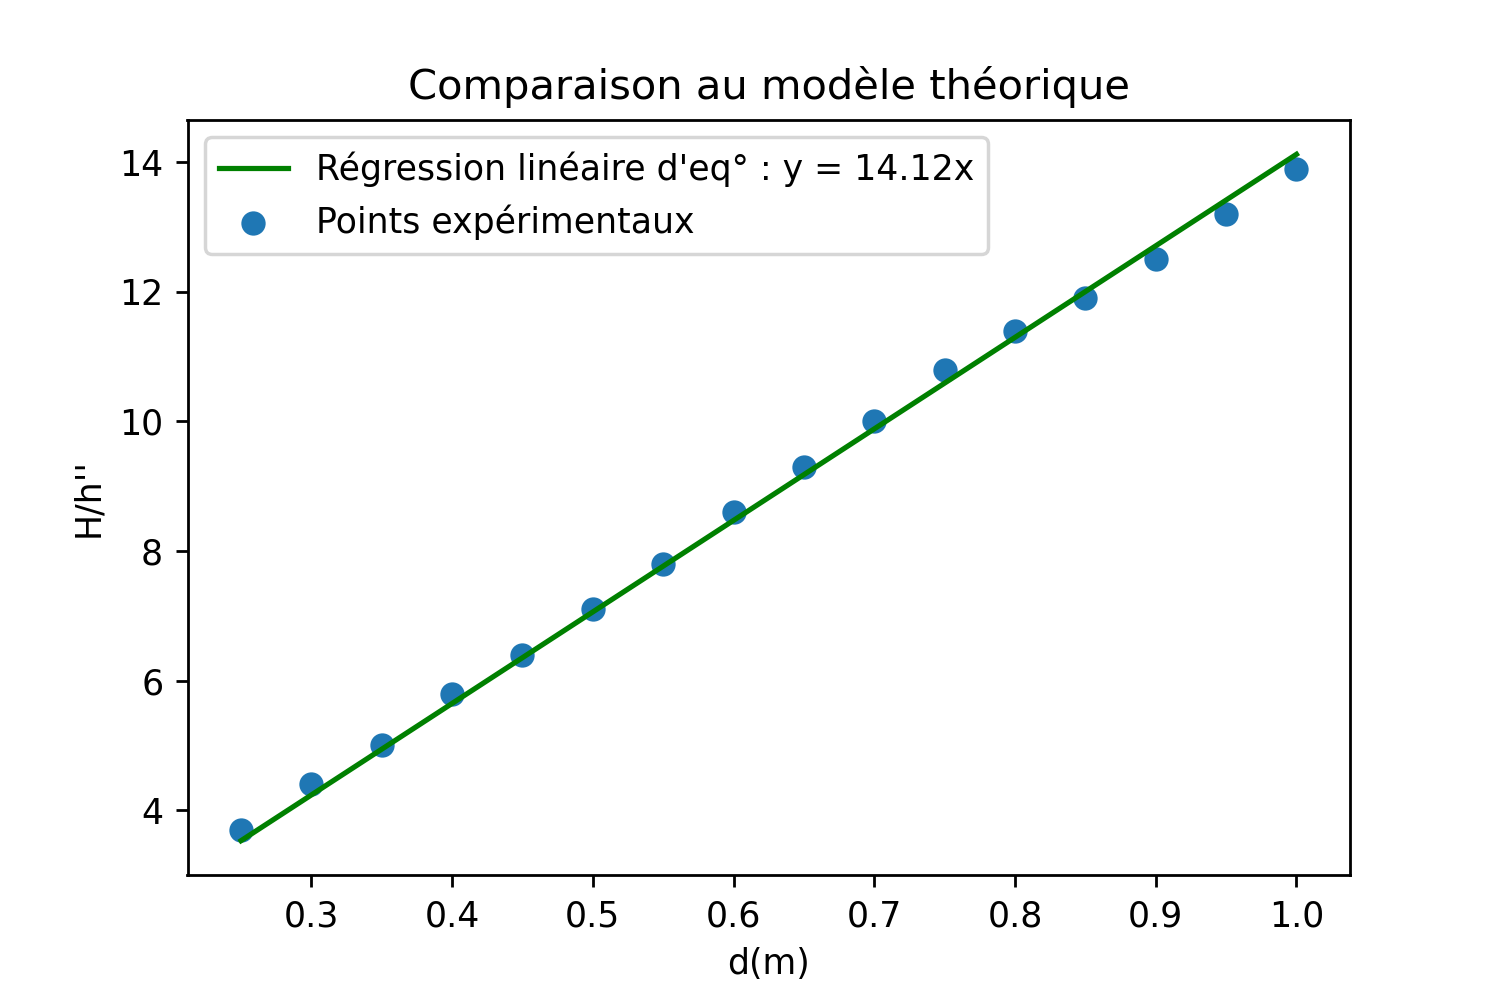
\includegraphics[scale=1]{Figures/opt}
\end{center}
\end{figure}


La pente correspondant à l'ajustement de nos données vaut : $14.12~m^{-1}$, calculons maintenant $K$ :
$$K=\frac{hc}{hef} = \frac{8.5\cdot 10{-3}}{13.97\cdot 10^{-2}\cdot4\cdot 10^{-3}}=15.21 ~m^{-1}$$\\
L'incertitude sur la pente nous est donnée par la matrice de covariance \textit{pcov} et vaut $\sigma = 3.14\cdot 10^{-4}~m^{-1}$. On obtient donc finalement : $$\boxed{K~=~(14.12 \pm 3.14\cdot10^{-4})m^{-1}}$$ Le coefficient de corrélation $\chi^{2}$ nous ait donné par le module \textit{scipy} et vaut 0.97, soit 97\%.\\

Nous pouvons à partir des informations récoltées lors du traitement de nos données, dire que le modèle décrit quantitativement les données expérimentales et ce de manière très pertinente en s'appuyant sur le coefficient de corrélation, le graphe, la pente calculée et celle déterminée d'après Python. Le modèle linéaire choisi traduit donc bien les variations de $H/h''$ en fontion de $d$.\\
Pour conclure, nous pouvons dire que l'appareil photo d'un smartphone peut être assimilé à une lentille mince.\\

Concernant les expériences réalisées, quelques précisions : \\

J'ai reproduis l'expérience chez moi, nous n'avions pas réalisé suffisamment de mesures lors du TP réalisé en classe. J'ai tenté cette fois de réduire au maximum les incertitudes, d'une part en faisant en sorte de ne pas trop fausser la mesure de $h''$ en utilisant un support perpendiculaire à la table et en faisant une quinzaine de mesures, ce qui me semble plus que raisonnable.
\end{document}
